\section{Method}

\subsection{Task definition}
Given a Vietnamese utterance $x$, ViPragSent predicts six binary pragmatic labels in the manifest order: implicit sentiment, sarcasm, irony, idiom/figurative language, code-switching, and mocking. These labels represent distinct pragmatic phenomena. The model may also predict a three-way polarity label and a seven-way emotion label. The auxiliary labels are not additional pragmatic classes.

For each pragmatic head, the metric is binary macro-F1: the arithmetic mean of the F1 values for class 0 and class 1. The macro-pragmatic F1 is the arithmetic mean of the six binary macro-F1 values. This definition is important for the head-level table because it differs from a positive-class-only F1.

\subsection{XLM-R-large encoder and prediction heads}

\begin{figure*}[t]
  \centering
  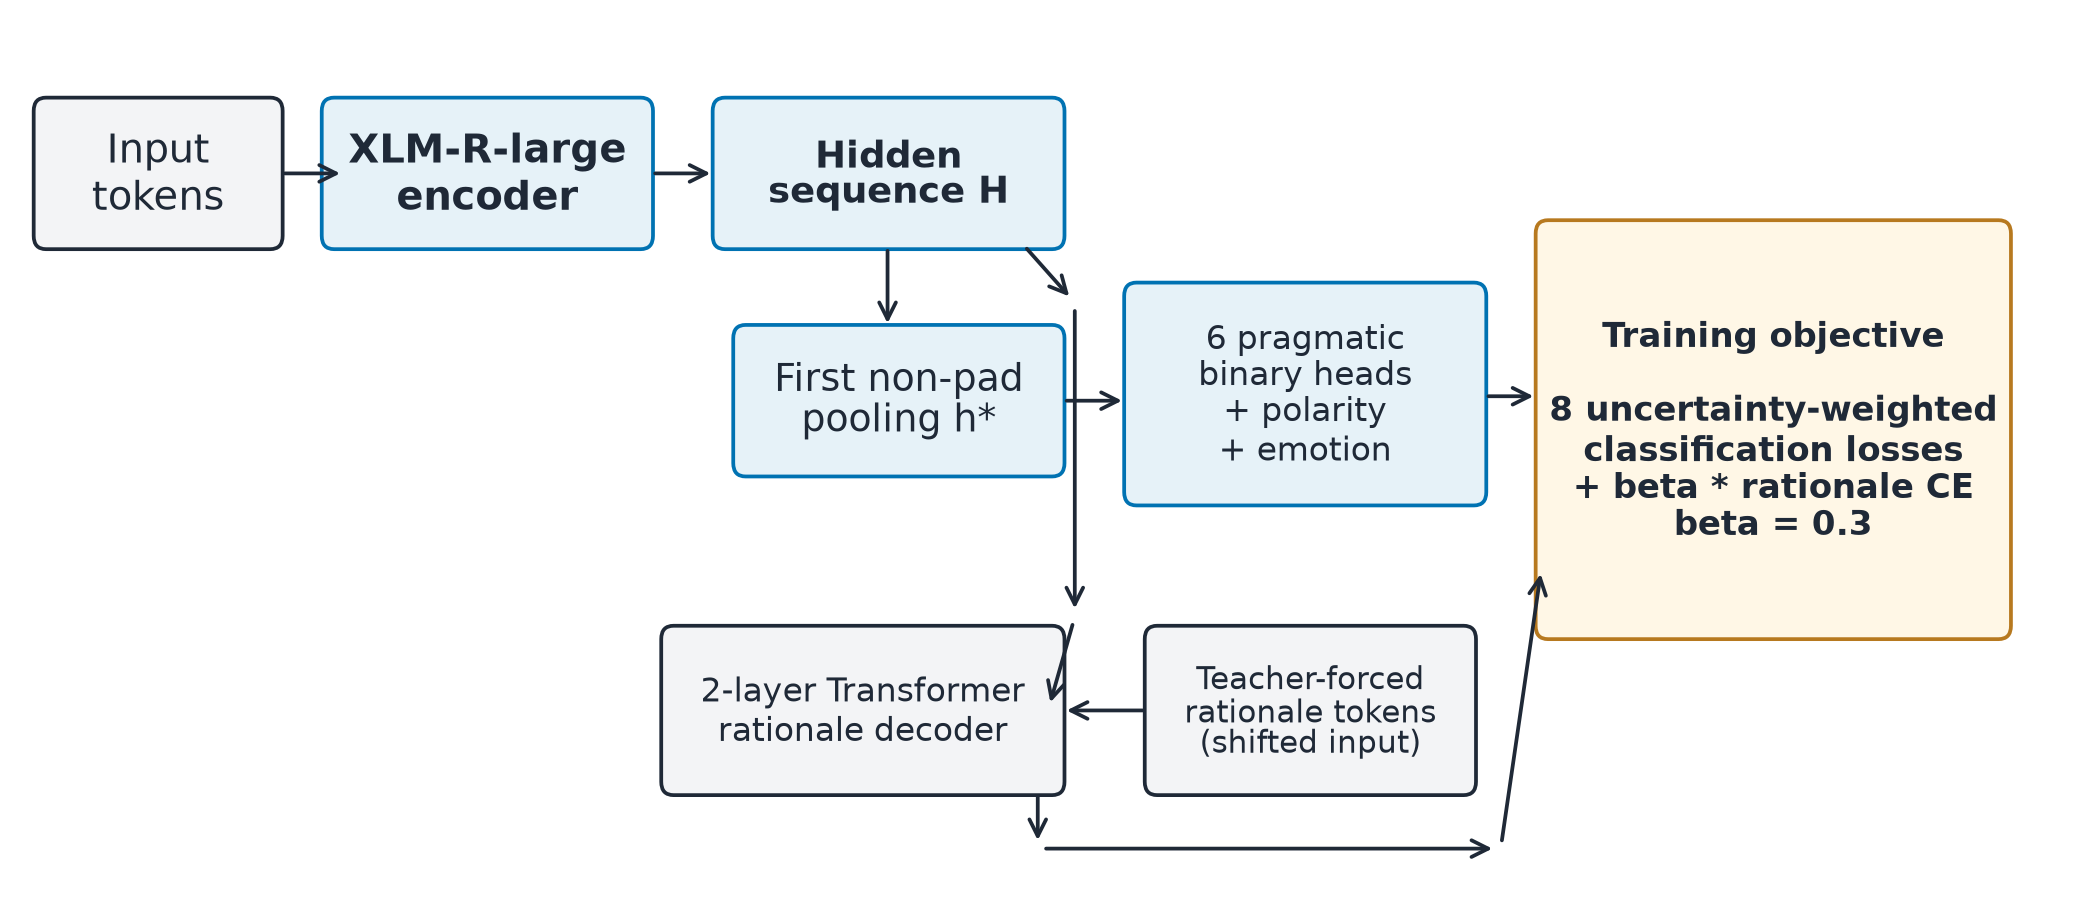
\includegraphics[width=\textwidth]{figures/figure_architecture_schematic.png}
  \caption{ViPragSent architecture and training objective. XLM-R-large produces a hidden sequence that feeds first-nonpadding pooling for six pragmatic binary heads, three-way polarity, and seven-way emotion prediction. The same hidden sequence is used as memory by a two-layer rationale decoder with teacher-forced shifted rationale tokens during training only; its rationale loss contributes to the objective and is not an inference output.}
  \label{fig:architecture}
\end{figure*}

The primary model uses \texttt{Facebook\allowbreak{}AI/xlm-r\allowbreak{}oberta-l\allowbreak{}arge} at revision \texttt{c23d21b0\allowbreak{}620b635a\allowbreak{}76227c60\allowbreak{}4d44e43a\allowbreak{}9f0ee389}. The encoder returns a hidden state for each input token. For the XLM-R family, the implementation pools the first nonpadding representation: the hidden state at the first position with an active attention mask, rather than a mean over the sequence. A 0.1 dropout layer feeds task-specific linear heads: six one-logit binary heads, one three-logit polarity head, and one seven-logit emotion head. At inference, predictions come from these classification heads.

\subsection{Implemented auxiliary objective}
The six pragmatic heads use weighted binary cross-entropy with logits, with positive-class weights computed from the training split. Polarity and emotion use class-weighted cross-entropy. For the full model, the eight classification losses have independent learned log-variance parameters. Let $\mathcal{T}$ be the eight classification tasks, let $m_t$ be the recorded task multiplier, and let $s_t$ be the learned log variance. The implementation clamps the log variance before applying uncertainty weighting:

\[
\begin{aligned}
s_t^{\mathrm{c}}=\operatorname{clip}(s_t,-5,5), \\
\mathcal{L}_{\mathrm{cls+rat}}=\sum_{t\in\mathcal{T}}\Bigl[\tfrac12 e^{-s_t^{\mathrm{c}}}(m_t\ell_t)+\tfrac12s_t^{\mathrm{c}}\Bigr] \\
{}+\beta\mathcal{L}_{\mathrm{rat}},\qquad \beta=0.3.
\end{aligned}
\]
Here $\ell_t$ is the task loss before the multiplier, so the multiplier is applied inside the uncertainty-weighted classification term. The rationale term is present only for the full rationale-enabled variant.

The rationale component is a two-layer causal \texttt{TransformerDecoder}. It uses a memory projection from the encoder hidden size to a decoder hidden size of 128, four attention heads, feed-forward size 512, dropout 0.1, causal masking, and tied token input/output embeddings. During training it consumes rationale tokens with teacher forcing and contributes token cross-entropy as $\beta\mathcal{L}_{\mathrm{rat}}$ with $\beta=0.3$. For the target run, the manifest identifies \texttt{approved\allowbreak{}\_generat\allowbreak{}ed\_ratio\allowbreak{}nales\_tr\allowbreak{}ain.json\allowbreak{}l} with 7,998 training rows. The inspected evidence does not identify a provider for these generated targets, so we treat this as a run-level training artifact rather than evidence about the original dataset's annotation history. The decoder is discarded from the inference path and produces no reported prediction.

\subsection{Training and selection}
The frozen ViPragSent package is identified in the data handoff as the SEACrowd/ViSoBERT source package and contains 11,997 rows: 7,998 training, 1,999 development, and 2,000 test examples. The split seed is 20260520. Training uses date-coded seeds 20260521, 20260522, and 20260523, reported in the paper as logical seeds 21, 22, and 23. The primary Q1a v37 configuration uses AdamW with learning rate $2\times10^{-5}$, weight decay 0.01, a maximum of 10 epochs, bf16 precision, physical batch size 8 with four accumulation steps (effective batch size 32), gradient clipping 1.0, cosine scheduling, and a 0.20 warmup ratio. Early stopping patience is 10. The primary loss multipliers are 1.01 for implicit sentiment, 1.01 for sarcasm, 1.05 for irony, and 1.04 for code-switching; the other task multipliers are 1.0. The selection metric is development macro-pragmatic F1.

For each binary pragmatic head, the development threshold is selected from 0.05 through 0.95 in steps of 0.01 by binary macro-F1, with ties resolved toward 0.5. Q3 applies this rule independently for each seed and budget. Q4 uses raw positive-class sigmoid probabilities and therefore does not threshold the probabilities before computing ECE.

For Q2, polarity ECE is the ten-bin top-label ECE computed from the saved development predictions and development metrics for each seed, then reported on the $10^3$ scale. The legacy field name \texttt{polarity\_dev\_ece} is retained for provenance; it does not indicate that the test-file value was used.

\subsection{Provenance and comparison scope}
The Q1a evidence package contains 18 saved prediction JSONL files: three ViPragSent target runs and three runs for each of five complete baseline families. Every one of the 45 target--baseline pairs has 2,000 rows with the same sample-ID set and the same six pragmatic gold-label tuples when aligned by sample ID. The Q1a scores were deterministically recomputed from those saved rows using the metric above. This supports a direct score comparison for the evaluated ID/gold cohort. It does not claim identical upstream input text, identical training, a significance test, or an independent rerun.
